% Hero image: Concept Comparison + Scaling Chart
% Top: GPU Full Scan vs PRISM (unchanged TikZ)
% Bottom: Throughput vs context length (pgfplots)
\documentclass[tikz,border=4pt]{standalone}

\usepackage{tikz}
\usetikzlibrary{calc, positioning, arrows.meta, fit, backgrounds, decorations.pathreplacing}
\usepackage{pgfplots}
\pgfplotsset{compat=1.18}

% ── Colour palette (Tier 1 universal) ──────────────────────────────
\definecolor{elecFill}{HTML}{E8E8E8}       % warm light gray — electronic
\definecolor{photFill}{HTML}{D4E4EC}        % pale blue-gray — photonic/hybrid
\definecolor{accentTeal}{HTML}{4DB8C7}      % cyan-teal accent
\definecolor{mrrBlue}{HTML}{BDD7E7}         % slightly deeper blue for MRR
\definecolor{pdFill}{HTML}{C8DDE6}          % blue-gray for photodetectors
\definecolor{queryFill}{HTML}{F0F0F0}       % very light gray for query
\definecolor{darkNavy}{HTML}{1B3A5C}        % dark navy
\definecolor{bottleneckRed}{HTML}{CC3333}   % red for GPU bottleneck arrows
\definecolor{selectiveBlue}{HTML}{66B2FF}   % sky blue for PRISM selective arrows
% Chart colors
\definecolor{prismBlue}{HTML}{2196F3}
\definecolor{questRed}{HTML}{F44336}
\definecolor{fullOrange}{HTML}{FF9800}
\definecolor{prismBlueDark}{HTML}{1565C0}
\definecolor{prismBlueLight}{HTML}{BBDEFB}

\begin{document}
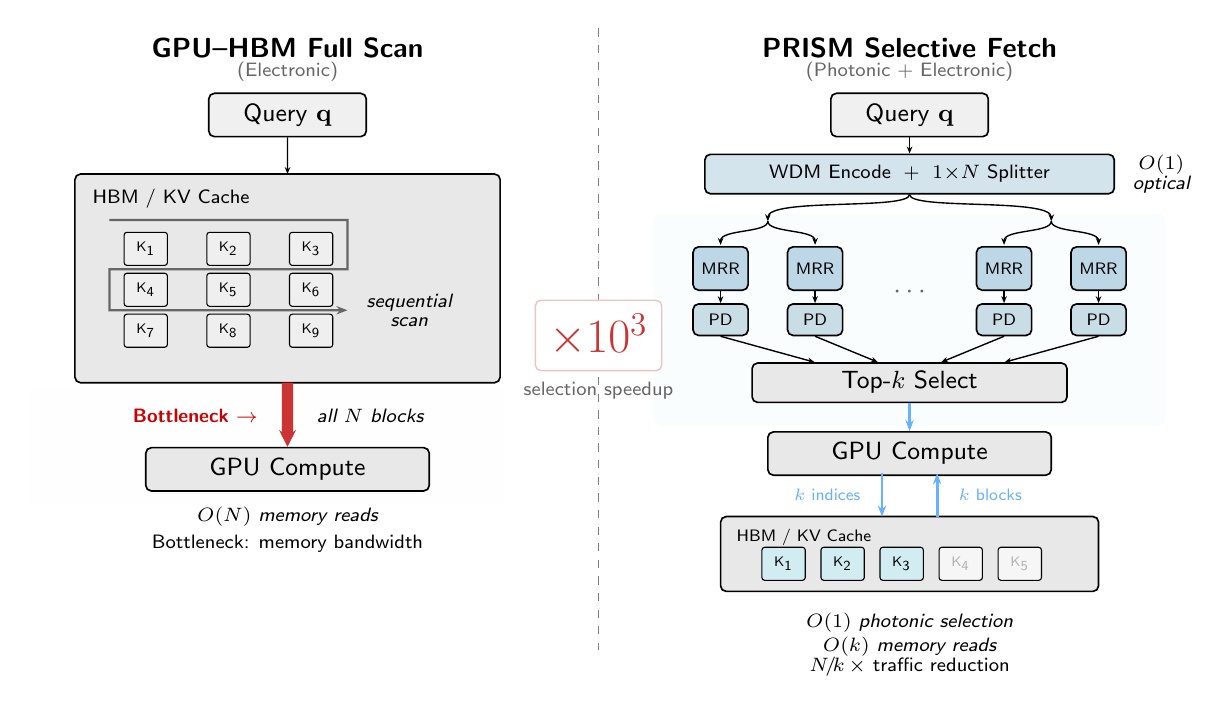
\begin{tikzpicture}[
    >=Stealth,
    font=\sffamily\small,
    % ── Block styles ───────────────────────────────────────────────
    stdbox/.style={
        rectangle, rounded corners=2pt,
        draw=black, line width=0.6pt,
        minimum height=0.55cm, text=black,
        inner sep=3pt, align=center,
    },
    querybox/.style={
        stdbox, fill=queryFill,
        minimum width=2.0cm,
    },
    elecbox/.style={
        stdbox, fill=elecFill,
    },
    photbox/.style={
        stdbox, fill=photFill,
    },
    mrrbox/.style={
        stdbox, fill=mrrBlue,
        minimum width=0.7cm, minimum height=0.55cm,
        font=\sffamily\fontsize{6}{7}\selectfont,
    },
    pdbox/.style={
        stdbox, fill=pdFill,
        minimum width=0.7cm, minimum height=0.4cm,
        font=\sffamily\fontsize{6}{7}\selectfont,
    },
    kvblock/.style={
        rectangle, rounded corners=1pt,
        draw=black, line width=0.4pt,
        minimum width=0.55cm, minimum height=0.42cm,
        inner sep=1pt, align=center,
        font=\sffamily\fontsize{5.5}{6.5}\selectfont,
    },
    annot/.style={
        font=\sffamily\itshape\fontsize{7}{8}\selectfont,
        text=black, align=center,
    },
    titlefont/.style={
        font=\sffamily\bfseries\normalsize,
        text=black,
    },
    arrowstyle/.style={
        -{Stealth[length=2.5pt, width=2pt]}, line width=0.5pt, black,
    },
]

% ====================================================================
% Geometry constants
% ====================================================================
\def\panelW{7.2}     % cm per panel
\def\gap{0.7}        % gap at center for dashed line
\def\leftX{0}
\pgfmathsetmacro{\rightX}{\panelW + \gap}
\pgfmathsetmacro{\midX}{\panelW + \gap/2}
\pgfmathsetmacro{\totalW}{2*\panelW + \gap}  % 15.1 cm

% ====================================================================
% LEFT PANEL — Electronic (GPU)
% ====================================================================
\begin{scope}[shift={(\leftX, 0)}]

    % ── Title ──────────────────────────────────────────────────────
    \node[titlefont] (ltitle) at (\panelW/2, 0.15) {GPU--HBM Full Scan};
    \node[font=\sffamily\fontsize{7}{8}\selectfont, text=black!60] at (\panelW/2, -0.15) {(Electronic)};

    % ── Query q ────────────────────────────────────────────────────
    \node[querybox] (lquery) at (\panelW/2, -0.7) {Query $\mathbf{q}$};

    % ── HBM / KV Cache label ABOVE the box ─────────────────────
    \coordinate (hbmTL) at (0.9, -1.45);
    \coordinate (hbmBR) at (\panelW - 0.9, -4.10);

    % HBM box drawn first
    \draw[rounded corners=2pt, draw=black, line width=0.6pt, fill=elecFill]
        (hbmTL) rectangle (hbmBR);

    % Label inside box, top-left
    \node[font=\sffamily\fontsize{7}{8}\selectfont, text=black, anchor=north west]
        at ($(hbmTL) + (0.1, -0.06)$) {HBM / KV Cache};

    % ── 3×3 grid of KV blocks ─────────────────────────────────────
    \foreach \row [count=\ri from 0] in {0,1,2} {
        \foreach \col [count=\ci from 0] in {0,1,2} {
            \pgfmathtruncatemacro{\idx}{\ri*3 + \ci + 1}
            \pgfmathsetmacro{\bx}{1.8 + \ci * 1.05}
            \pgfmathsetmacro{\by}{-2.40 - \ri * 0.52}
            \node[kvblock, fill=elecFill!70!white] (lkv\idx) at (\bx, \by)
                {K\textsubscript{\idx}};
        }
    }

    % ── Snake-scan arrow through KV grid rows ──
    \draw[arrowstyle, line width=0.8pt, black!60,
          -{Stealth[length=4pt, width=3pt]}]
        ($(lkv1.north west) + (-0.18, 0.15)$)
        -- ($(lkv3.north east) + (0.18, 0.15)$)
        -- ($(lkv3.south east)!0.5!(lkv6.north east) + (0.18, 0)$)
        -- ($(lkv1.south west)!0.5!(lkv4.north west) + (-0.18, 0)$)
        -- ($(lkv4.south west)!0.5!(lkv7.north west) + (-0.18, 0)$)
        -- ($(lkv6.south east)!0.5!(lkv9.north east) + (0.18, 0)$);

    \node[annot, anchor=west] at ($(lkv6.south east)!0.5!(lkv9.north east) + (0.30, 0)$)
        {sequential\\[-1pt]scan};

    % ── GPU Compute box ───────────────────────────────────────────
    \node[elecbox, minimum width=3.6cm] (lgpu)
        at (\panelW/2, -5.20) {GPU Compute};

    % ── Bottleneck background ────────────
    \begin{scope}[on background layer]
        \fill[black!15, opacity=0.03, rounded corners=3pt]
            ($(hbmBR) + (-6.0, -0.05)$) rectangle ($(lgpu.south -| hbmBR) + (0.05, -0.15)$);
    \end{scope}

    % ── Thick bottleneck arrow ──
    \draw[-{Stealth[length=6pt, width=6pt]}, line width=4pt, bottleneckRed]
        ($(hbmBR)!0.5!(hbmBR -| hbmTL) + (0, 0)$) -- (lgpu.north);
    \node[annot, anchor=west] at ({\panelW/2 + 0.25}, {(-4.10 + -5.20 + 0.25) / 2})
        {all $N$ blocks};
    \node[annot, font=\sffamily\bfseries\fontsize{7}{8}\selectfont, text=red!80!black, anchor=east]
        at ({\panelW/2 - 0.25}, {(-4.10 + -5.20 + 0.25) / 2})
        {Bottleneck $\rightarrow$};

    % ── Arrow from query to HBM ──────────────────────────────────
    \draw[arrowstyle] (lquery.south) -- ($(hbmTL)!0.5!(hbmTL -| hbmBR) + (0, 0)$);

    % ── Annotations ─────────────────────────────────────────────
    \node[annot, font=\sffamily\itshape\fontsize{7.5}{9}\selectfont]
        at (\panelW/2, -5.80)
        {$O(N)$ memory reads};
    \node[annot, font=\sffamily\fontsize{7}{8}\selectfont, text=black]
        at (\panelW/2, -6.15)
        {Bottleneck: memory bandwidth};

\end{scope}

% ====================================================================
% DASHED DIVIDER
% ====================================================================
\draw[dashed, black!50, line width=0.5pt]
    (\midX, 0.4) -- (\midX, -7.5);

% ── Big improvement annotation on divider ──
\node[fill=white, rounded corners=2pt, inner sep=5pt,
      font=\sffamily\bfseries\LARGE,
      text=bottleneckRed, draw=bottleneckRed!30, line width=0.5pt]
    at (\midX, -3.5) {$\boldsymbol{\times 10^3}$};
\node[font=\sffamily\fontsize{7}{8}\selectfont, text=black!60]
    at (\midX, -4.2) {selection speedup};

% ====================================================================
% RIGHT PANEL — PRISM (Photonic)
% ====================================================================
\begin{scope}[shift={(\rightX, 0)}]

    \node[titlefont] (rtitle) at (\panelW/2, 0.15) {PRISM Selective Fetch};
    \node[font=\sffamily\fontsize{7}{8}\selectfont, text=black!60] at (\panelW/2, -0.15) {(Photonic + Electronic)};

    \node[querybox] (rquery) at (\panelW/2, -0.7) {Query $\mathbf{q}$};

    \node[photbox, minimum width=5.2cm, minimum height=0.50cm,
          font=\sffamily\fontsize{7.5}{8.5}\selectfont]
        (rwdm) at (\panelW/2, -1.45)
        {WDM Encode\; +\; $1{\times}N$ Splitter};
    \draw[arrowstyle] (rquery.south) -- (rwdm.north);
    \node[annot, anchor=west] at ($(rwdm.east) + (0.1, 0)$)
        {$O(1)$\\[-1pt]optical};

    \begin{scope}[on background layer]
        \fill[accentTeal, opacity=0.03, rounded corners=3pt]
            (0.35, -1.95) rectangle (\panelW - 0.35, -4.65);
    \end{scope}

    \def\numChan{4}
    \def\chanA{1.2}
    \def\chanB{2.4}
    \def\chanC{4.8}
    \def\chanD{6.0}

    \pgfmathsetmacro{\splitMidX}{\panelW/2}
    \def\splitLy{-2.05}
    \pgfmathsetmacro{\groupLx}{(\chanA + \chanB) / 2}
    \pgfmathsetmacro{\groupRx}{(\chanC + \chanD) / 2}
    \draw[arrowstyle] (rwdm.south)
        .. controls ++(0, -0.2) and ++(0, 0.3) .. (\groupLx, \splitLy);
    \draw[arrowstyle] (rwdm.south)
        .. controls ++(0, -0.2) and ++(0, 0.3) .. (\groupRx, \splitLy);

    \draw[arrowstyle] (\groupLx, \splitLy)
        .. controls ++(0, -0.15) and ++(0, 0.2) .. (\chanA, -2.35);
    \draw[arrowstyle] (\groupLx, \splitLy)
        .. controls ++(0, -0.15) and ++(0, 0.2) .. (\chanB, -2.35);
    \draw[arrowstyle] (\groupRx, \splitLy)
        .. controls ++(0, -0.15) and ++(0, 0.2) .. (\chanC, -2.35);
    \draw[arrowstyle] (\groupRx, \splitLy)
        .. controls ++(0, -0.15) and ++(0, 0.2) .. (\chanD, -2.35);

    \foreach \c/\cx in {1/\chanA, 2/\chanB, 3/\chanC, 4/\chanD} {
        \node[mrrbox] (mrr\c) at (\cx, -2.65) {MRR};
        \node[pdbox] (pd\c) at (\cx, -3.30) {PD};
        \draw[arrowstyle] (mrr\c.south) -- (pd\c.north);
    }

    \node[font=\sffamily\fontsize{10}{11}\selectfont, text=black!60]
        at ({(\chanB + \chanC) / 2}, -2.95) {$\cdots$};

    \node[elecbox, minimum width=4.0cm, minimum height=0.5cm]
        (rtopk) at (\panelW/2, -4.10) {Top-$k$ Select};

    \foreach \c [count=\ci from 1] in {1,...,\numChan} {
        \draw[arrowstyle] (pd\c.south) -- ($(rtopk.north west)!\ci/5!(rtopk.north east)$);
    }

    \node[elecbox, minimum width=3.6cm] (rgpu)
        at (\panelW/2, -5.00) {GPU Compute};

    \draw[-{Stealth[length=4pt, width=3pt]}, line width=1.2pt, selectiveBlue]
        (rtopk.south) -- (rgpu.north);

    \coordinate (rhbmTL) at (1.2, -5.80);
    \coordinate (rhbmBR) at (\panelW - 1.2, -6.75);

    \draw[rounded corners=2pt, draw=black, line width=0.6pt, fill=elecFill]
        (rhbmTL) rectangle (rhbmBR);

    \node[font=\sffamily\fontsize{6.5}{7.5}\selectfont, text=black, anchor=north west]
        at ($(rhbmTL) + (0.08, -0.04)$) {HBM / KV Cache};

    \pgfmathsetmacro{\rkStart}{2.0}
    \foreach \b [count=\bi from 0] in {1,...,5} {
        \pgfmathsetmacro{\bx}{\rkStart + \bi * 0.75}
        \ifnum\b<4
            \node[kvblock, fill=accentTeal!25] (rkv\b) at (\bx, -6.40)
                {K\textsubscript{\b}};
        \else
            \node[kvblock, fill=elecFill!40!white, text=black!30] (rkv\b)
                at (\bx, -6.40) {K\textsubscript{\b}};
        \fi
    }

    \draw[-{Stealth[length=4pt, width=3pt]}, line width=1.0pt, selectiveBlue]
        ({\panelW/2 - 0.35}, -5.25) -- ({\panelW/2 - 0.35}, -5.80);
    \draw[-{Stealth[length=4pt, width=3pt]}, line width=1.0pt, selectiveBlue]
        ({\panelW/2 + 0.35}, -5.80) -- ({\panelW/2 + 0.35}, -5.25);
    \node[annot, anchor=east, font=\sffamily\fontsize{6}{7}\selectfont, text=selectiveBlue]
        at ({\panelW/2 - 0.50}, -5.52)
        {$k$ indices};
    \node[annot, anchor=west, font=\sffamily\fontsize{6}{7}\selectfont, text=selectiveBlue]
        at ({\panelW/2 + 0.50}, -5.52)
        {$k$ blocks};

    \node[annot, font=\sffamily\itshape\fontsize{7.5}{9}\selectfont]
        at (\panelW/2, -7.15)
        {$O(1)$ photonic selection};
    \node[annot, font=\sffamily\itshape\fontsize{7.5}{9}\selectfont]
        at (\panelW/2, -7.45)
        {$O(k)$ memory reads};
    \node[annot, font=\sffamily\fontsize{7}{8}\selectfont, text=black]
        at (\panelW/2, -7.70)
        {$N\!/\!k\,\times$ traffic reduction};

\end{scope}

% Chart is appended by make_hero_v2.py from paper matplotlib figure

\end{tikzpicture}
\end{document}
